%Templated from IEEE Preparation Papers
\documentclass[letterpaper, 10 pt, conference]{ieeeconf}
\usepackage{graphicx}
\IEEEoverridecommandlockouts                              % This command is only
                                                          % needed if you want to
                                                          % use the \thanks command
\overrideIEEEmargins
% See the \addtolength command later in the file to balance the column lengths
% on the last page of the document

% The following packages can be found on http:\\www.ctan.org
\usepackage{graphics} % for pdf, bitmapped graphics files
\usepackage{epsfig} % for postscript graphics files
\usepackage{mathptmx} % assumes new font selection scheme installed
\usepackage{times} % assumes new font selection scheme installed
\usepackage{amssymb}  % assumes amsmath package installed
\usepackage{amsmath}
\title{\LARGE \bf
Workload  Management  in  Multicore  Processing 
}

\author{ \parbox{3 in}{\centering Will Wu\\
        Electrical and Computer Engineering\\
        University of Rochester\\
        500 Computer Studies Building \\
        Rochester, NY 14627\\
        {\tt\small ywu37@ur.rochester.edu}}
}

\begin{document}

\maketitle
\thispagestyle{empty}
\pagestyle{empty}



%%%%%%%%%%%%%%%%%%%%%%%%%%%%%%%%%%%%%%%%%%%%%%%%%%%%%%%%%%%%%%%%%%%%%%%%%%%%%%%%
\section{INTRODUCTION}

Queues are ubiquitous in our consumerist way of life.  Every economic transaction is explained by analyzing supply and demand curves.  An athlete needs a new pair of shoes.  A battery powered device needs a new set of batteries to function.  A mother orders from a takeout restaurant for the entire family.  In all three of the previous scenarios, a customer demands a service and enters the queueing system to be serviced or have its demand satisfied by any one of the servers provided by the service and then exits the queueing system.  A queueing line most prominently appears when the rate of customer arrivals demanding a service and the rate of customers being serviced is not identical.

In the realm of computer architecture, the proliferation of multicore processing systems in an attempt to execute multiple different programs on multiple different datasets has been a compelling reason to tie in the study of graph theory. With the introduction of more unsynchronized cores, communication among those cores is necessary to ensure unnecessary excess work is performed, bloating execution time.  The use of queues are necessary to hold metadata that allows for cross-core communication and synchronization.  For the purposes of this paper, the term "core" is not restricted to a computation core soldered onto a microprocessor.  It is used to generally talk about a device that is accomplishing work in the realm of program execution.  This ranges from as small as an arithmetic logic unit running a reduced instruction set architecture to a graphics processing unit working a large image dataset to as large as a large server room handling database queries or TCP connections and everything in between.

\section{THE NATURE OF MULTICORE PROCESSING}

Before diving into the study of how graph and queue theory can help in the design of multicore processors, it is helpful to define some terms from computer architecture.  Latency is defined as the time differential between a customer entering a system and that customer leaving the system.  This is also referred to as the sojourn time in the realm of graph theory.  Throughput defined as the amount of work done over some period of time. This paper will focus on the three components of interconnect design are topology, routing, and flow control.   The term topology relates to the geometric structure of the network: the relationship between nodes and wires connecting those nodes.  This is the most visual portion of design and relates closely with graph theory.  The term routing relates to the algorithms that dictate the protocol of how packets traverse through the network.  Flow control has to do with the resources of the network and how they are used to allow packets of datagrams to traverse through the network.  Flow control is much less associated with the topology of a network whereas routing is immensely affected by the network's topology.  Routing is a programmable algorithm of getting a packet from a source node to a destination node.  Flow control consist of the hardware components that is part of the interconnect.  Topology dictates exactly which nodes the flow control connects.

\begin{figure}[!ht] %Queue Model
	\centering
	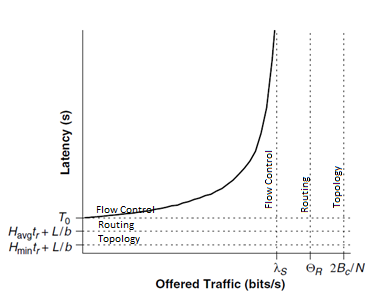
\includegraphics [width=0.5\textwidth] {Traffic_vs_Latency.png} 
    \caption{The cumulative effects of Topology, Routing, and Flow Control on the latency of packet movement.}
\end{figure}


The interconnection network is the name given for the system of programmable devices that handles communications between many different terminals.  For the most part, these terminals correspond with a processing core on the chip while some terminals are dedicated to the memory system or the input/output ports.  Such an organization scheme is shown in the figure below.  It is important to note that the interconnect does not necessarily have to connect every port to every other port.  Low latency is more difficult as the number of nodes scale up, the amount of space the wiring between devices grows more slowly than the expected traffic through those wires [19].

\begin{figure}[!ht] %Mesh Bisection
	\centering
	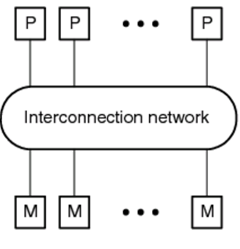
\includegraphics[width=0.5\textwidth] {Interconnect.png} 
    \caption{The interconnection network in relation to processing cores ports and memory ports [1]}
\end{figure}

The bisection bandwidth is one of the most important characteristics in the design of interconnect.  It is defined as the minimum bandwidth of all bisections of a network and approximately 50\% of the traffic through a network traverses through that bisection [1].  The bisection bandwidth is outlined in the figure below.  With the current design paradigm, the bisection area grows at a scale of $N^{2/3}$ while the traffic grows by a scale of N nodes [19].  

\begin{figure}[!ht] %Mesh Bisection
	\centering
	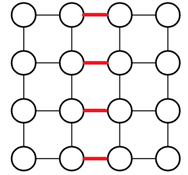
\includegraphics [width=0.5\textwidth] {Mesh_Bisection_Bandwidth.png} 
    \caption{The bisection bandwidth of this 4-ary 2-cube network is outlined in red.}
\end{figure}

There are many different ways to organize processing cores among themselves.  The simplest interconnect topology between especially small number of cores is a bus topology where every port to every other port .  A ring topology can be thought of a bus topology with its two ends tied together. In a ring interconnect system, every port is no longer required to be connected to every other port in the system.  Neighboring nodes communicate with each other.  A mesh topology is a grid layout of nodes with immediate neighbor communication capabilities and is not restricted to two dimensions.  In a two-dimension mesh network, the entire network can be modeled with a Cartesian plane.  In a three-dimensional mesh network, the entire network can be modeled with a cube.  A torus topology is a mesh topology with its ends wrapping on itself.  A common everyday model for the torus network is a donut.  Torus networks are quite prevalent in present-day designs.  It has been found that torus networks always gives the lowest latency due to the highest bandwidth channels and most direct physical route between two nodes.  While higher-dimensional figures is a good method of understanding the structure of the topology in question, one discrepancy between the model and the development of the network topology is the realization that everything must be laid out on silicon which is typically in a two-dimensional plane.  To illustrate this point, the connections between ports of neighboring nodes are shown in the figure below.  

There is a naming convention for interconnects by indicating a networks dimensionality, topology, and radix.  A network of N nodes can be organized into a ${k}^{n}$ structure where k is the radix and n is the dimension.  This information is then compressed in two terms called k-ary n-naming convention.  The term after the 'n' describes the topology of the network.  For example: a 4-ary 2-cube network is a mesh network of radix 4 in 2 dimensions which is shown in the figure above.  When wire cost is considered, low dimensional networks such as torus networks offer lower latency than high dimensional networks such as binary n-cubes.

\begin{figure}[!ht] %Wiring a torus network
	\centering
	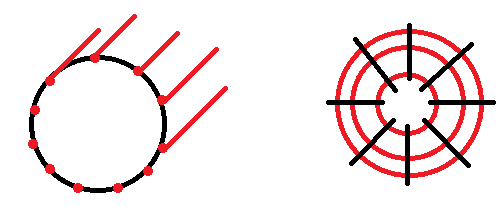
\includegraphics [width=0.5\textwidth] {Torus.png} 
    \caption{A ring of rings is a good way of visualizing a donut or torus network.}
\end{figure}


\begin{figure}[!ht] %Wiring a torus network
	\centering
	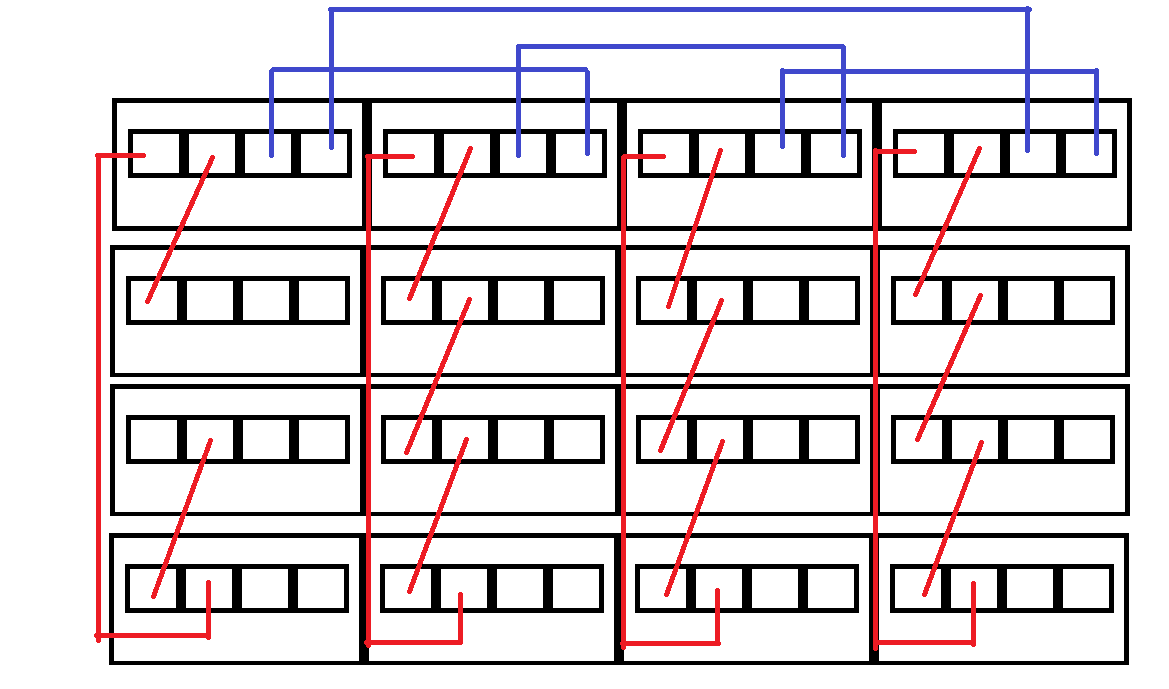
\includegraphics [width=0.5\textwidth] {torus_wiring.png} 
    \caption{Wiring a torus network (not all blue wires are shown as to not clutter the figure)}
\end{figure}


One fundamental aspect of program execution is that the number of requests present mid-execution at any one time cannot be negative.  Such a behavior can also be called a birth-death process.  This is where the study of queueing theory is invaluable. %FIN

\section{QUEUEING THEORY}

Now that a connection has been made between customers in a queue and threads and requests from processes, we can break down the anatomy of a queueing system.  A queue has three main attributes: the customer arrival rate, the customer departure rate or service rate, and the number of servers.  All other attributes can be derived from the first three attributes.  In the realm of computer processing, customers are thread and process requests or the working dataset.

\vspace{5mm}

The most common arrival distribution follows that of a Poisson distribution whereas the most common service distribution exponential distribution [2].  The rate of service for a queue behaves in an exponentially distributed manner with no regard to the service of other customers.  Given the nonidentical behaviors of the job arrival rate and job service rate, it is quite necessary for queues to be implemented for each node.

\begin{figure}[!ht] %Queue Model
	\centering
	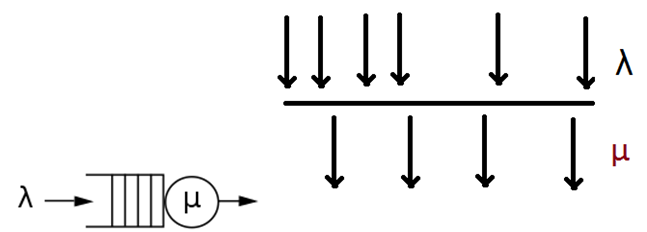
\includegraphics [width=0.5\textwidth] {Queue_Model.png} 
    \caption{A visualization of the queue model.  lambda represents the arrival rate and mu represents the service rate.}
\end{figure}

In the realm of queueing theory, Kendall's notation is a standardized method of describing different queues.  The M/M/1 queue structure is a good introduction to queueing theory and some time will be dedicated to talking about the other characteristics of the queue structure in the context of the M/M/1 queue.  The 'M' stands for the Markovian process that arrivals behave in.  As such, the rate of arrivals can be modeled by the following probability density function:

\begin{equation}
f(t) = \lambda e^{-\lambda t}\\
\end{equation}

The probability that the number of customers in the queue is less than X at any point after time t can derived from the following:

\begin{equation}
P(t,t= \Delta t | t > t_0) = \frac{\lambda e^{-\lambda t}} { \int_{t_0}^{\infty} \lambda e^{-\lambda t} dt} = \frac {\lambda e^{-\lambda t}}{e^{-\lambda t_0}} = \lambda e^{-\lambda (t-t_0)}
\end{equation}

\begin{table}
  \centering
    \begin{tabular}{|c|}
    \hline
    Kendall’s Notation: A/S/c/K/N/D \\
    \hline
A = time between arrivals \\
S = size of jobs \\
c = number of servers \\
K = capacity of queue \\
N = size of population of jobs to be served \\
D = queueing discipline \\
    \hline
    \end{tabular}
  \caption{Kendall's Notation}
\end{table}

When the final three parameters are not specified, K = $\infty$ N = $\infty$ and D = first in first out (FIFO) \footnote{first in first out (FIFO) can also be referred to as first come first serve (FCFS)} by convention.  The Kendall notation is very useful for modeling the queue but for realistic workload scenarios, K is bounded by the size of memory reserved and N is bounded by the number of requests.  The queueing discipline may not be a FIFO scheme for stack or recursive based workloads or priority based workloads.

Server utilization is only moderately important for the purposes of scaling up the workload.  Low server utilization may suggest imbalanced load assignment.  The average service time is one aspect that contributes to aggregate execution time.  The service time has been rigorously minimized over the years.  The more important time metric is the customer wait time.  This is because changes made to the interconnect vastly affects the skew between the customer arrival distribution and the customer service distribution.

\begin{equation}
\rho = \lambda T_s
\end{equation}

%MAKE INTO FORMULA
The steady state average number of customers in the queue is the product of the steady state arrival rate and the average time a customer spends in queue and in execution.  This simple relationship known as the Little's Law is independent of the service distribution or the method that requests enter the queueing system.

\begin{equation}
L = \lambda T_q = \frac{\rho}{(1-\rho)}
\end{equation}

\begin{equation}
P(n>=N) = \rho ^{n}
\end{equation}

\section {ADJUSTMENTS TO THE TORUS} 
Network pruning involves removing some of the links such that the network is not fully connected in accordance with the donut model.  Directed One idea is to permit single directional routing.  Due to both the directed nature of the network, the network diameter is no longer akin to that of a ring topology.  Due to the routing restriction, the team also had to compute the network diameter which is the maximum distance between any combination of two nodes in the network.  Pruning also influences latency in the aspect of hop count, or the number of intermediate nodes that a packet must traverse between source and destination node.
 
Parhami et al. clearly outlined their torus network Tera multithreaded architecture with the following adjacency matrix $\Omega$, pruning matrix $\Psi$.  Sets a and b consists of all nodes in the network and g is some element in the adjacency matrix and  $\Psi$ is derived by b = a +  $\Psi$$\Pi$$\Phi$g.  Directed matrix were construed using the adjacency matrix $\Omega$ and inversing all negative values of the orientation matrix. [17]

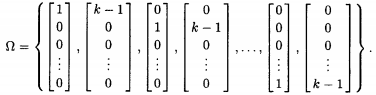
\includegraphics [width=0.5\textwidth] {Omega.PNG} 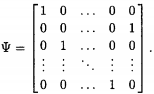
\includegraphics {Psi.PNG} 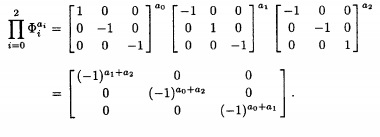
\includegraphics[width=0.5\textwidth] {Phi.PNG}

It was found that the pruning mechanism helped lower message latency with undirected connections.  The directionality of the connections provide some improvement in the unpruned networks but pruning those networks causes the routing to be too restrictive and worsens the latency under heavy loads.

\begin{figure}[!ht] %The four prune/directed torus network combinations
	\centering
	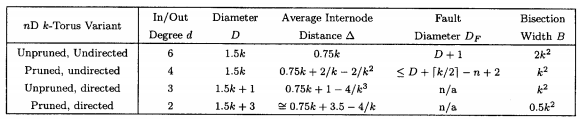
\includegraphics [width=0.5\textwidth] {Torus_Prune_Table2.PNG} 
    \caption{The performance models of 3D torus networks [17]}
\end{figure}

\begin{figure}[!ht] %The four prune/directed torus network combinations
	\centering
	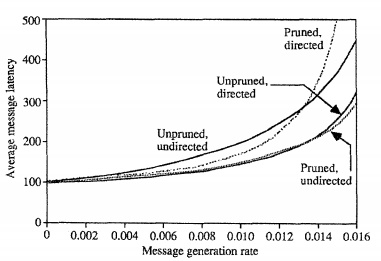
\includegraphics [width=0.5\textwidth] {Prune_Data.PNG} 
    \caption{Message latency with radix 16, message length 384 bytes [17]}
\end{figure}

\section{VARIOUS CASE STUDIES}
\subsection{The Butterfly Topology}

A butterfly topology is a simpler version of a mesh topology.  Nodes feed into (n-1) routers with a fan-in of k ports and a fan-out of k ports.  The butterfly network is most commonly used for Internet routing as it is the most scalable with n stages of routing devices for $k^{n}$ end user nodes.  The routing protocol is very simple as it involves computing the hamming distance between source and destination nodes.  The distance dictates the number of switching made during the packet's journey through the crossbar switch in each router.  The latency is has the least variance with every end node being equidistant from every other end node.  As such the hop count is incredibly low. %fin

\subsection{Task Assignment Schemes}

As a reminder, the processor sharing discipline is a queue discipline that is part of the Kendall's queue notation (under the letter representation 'D') explained earlier in the paper.  By default, a queue's discipline is FIFO.  Dynamic Task Allocation such as Processor Sharing is modeled under a M/G/1 queue (where G stands for geometric distribution).

\begin{figure}[!ht] %Dynamic Task Allocation PS
	\centering
	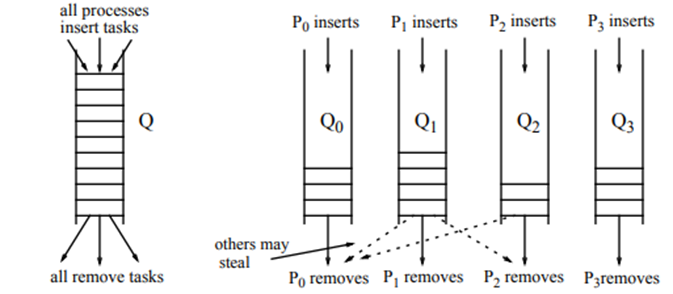
\includegraphics [width=0.5\textwidth] {Task_Snooping.png} 
    \caption{Dynamic Task Allocation through Task Snooping [3]}
\end{figure}

A method different from the task snooping explained above is increasing the redundancy of the work done.  At first glance this may seem wasteful but this method is used for big data computing using remote servers, where powerful hardware is not the limiting factor and timing is [16].  Tasks are assigned to multiple different cores with the core who completes the task first invalidating all other cores also completing the same task.  

\begin{figure}[!ht] %Dynamic Task Allocation PS
	\centering
	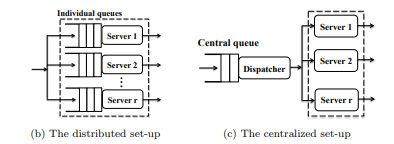
\includegraphics [width=0.5\textwidth] {Distr_vs_Centralized_Servers.PNG} 
    \caption{Distributed vs Centralized Redundant Task Allocation [3]}
\end{figure}

\subsection{SGI}

The SGI Origin server machine utilizes a cube and hypercube topology.  When the network is not fully saturated, it has the capability to utilize the hypercube's idle resources to effectively decrease the network diameter.  This at best cuts down the time spent in queue by half.  This sort of detection is CrayLink interconnect found in each node.  The SGI also uses a dynamic router and flow control mechanism called the wavefront allocator [4].  This allocator assigns all tasks in waves across the interconnect mesh.  A set of nodes are assigned together if they are equidistant from a local source node.  The task arbitration is done independently from previous or future stages.  This allocation technique allows for the latency to scale logarithmically with respect the number of nodes or linearly with the network diameter.

\begin{figure}[!ht] %Queue Model
	\centering
	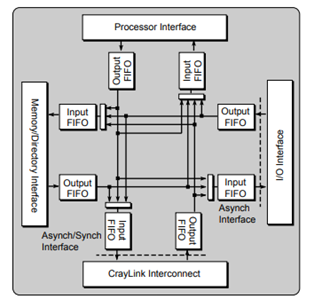
\includegraphics [width=0.5\textwidth] {CrayLink.png} 
    \caption{The CrayLink detection module in each node.}
\end{figure}

\section{FINAL REMARKS}

Throughout the research procedure in this deep pool of knowledge, development in the areas of interconnect can be broadly split into two categories.  The pruned torus networks from Parham et al. provide a design where specific connections between nodes are intentionally missing.  The directionality of torus networks restricts the movement of packets from bidirectional to unidirectional.  One the other end of the spectrum, some designs such as that of the SGI provide redundancy through increased circuitry.  Qui et al. also disseminated increased redundancy to make up for server failure rates.  So it can be generalized that network development has a conservative approach (where routing is restricted and more formulaic)  and a liberal approach (where multiple different path possibilities are viable).

It bears repeating but engineering has always been about cost/benefit analysis.  There can never be a design where the network interconnect is both reduced from that of the model and more redundant than the model.  The industry can never have its cake and eat it too.  So there must be a prescriptive approach to problem solving; different problems require different types of networks solutions.  A more conservative approach is to be used  on a specialized workload or where the routing algorithm is less reliable.  This comes at the expense of latency and overall time spent executing for execution correctness.  A more liberal approach can work where timing is more demanding and any inaccuracies in execution are tolerated or can be corrected before program termination.

\begin{figure}[!ht] %Extra Fly
	\centering
	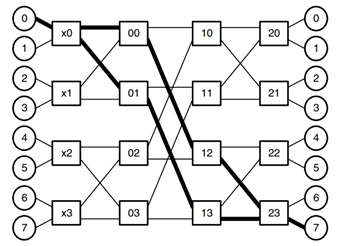
\includegraphics [width=0.5\textwidth] {Extra_Fly.png} 
    \caption{Adding an extra stage to this butterfly network allows for increased path diversity. [1]}
\end{figure}

\begin{figure}[!ht] %N/2 Stage Fly
	\centering
	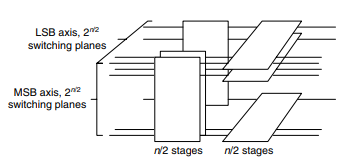
\includegraphics [width=0.5\textwidth] {Perpendicular_Planes_Butterfly.PNG} 
    \caption{The Construction of a Butterfly Network using Perpendicular Planes [1].}
\end{figure}

\addtolength{\textheight}{-12cm}   % This command serves to balance the column lengths
                                  % on the last page of the document manually. It shortens
                                  % the textheight of the last page by a suitable amount.
                                  % This command does not take effect until the next page
                                  % so it should come on the page before the last. Make
                                  % sure that you do not shorten the textheight too much.


\begin{thebibliography}{99}

\bibitem{c1} “Principles and Practices of Interconnection Networks”, By Dally and Towles, Morgan Kaufmann 2004. 

\bibitem{c2} “Parallel Computer Organization and Design”, Dubois, Annavaram, and Stenstrom. Cambridge University Press 2012.

\bibitem{c3} "Parallel computer architecture a hardware/software approach" D. Culler, J. Singh, and A. Gupta. , 1999.

\bibitem{c4} James Laudon and Daniel Lenoski. The SGI origin: A ccNUMA highly scalable server. In Proceedings of the 24th Annual International Symposium on Computer Architecture (ISCA-97), volume 25,2 of Computer Architecture News, pages 241–251, New York, June2– 4 1997. ACM Press.

\bibitem{c5} Daniel F. Spulber; Christopher S. Yoo, On the Regulation of Networks as Complex Systems: A Graph Theory Approach, 99 Nw. U. L. Rev. 1687 (2005)

\bibitem{c6} C. Guo, H. Wu, K. Tan, L. Shiy, Y. Zhang, and S. Lu. Bcube: A high performance, server-centric network architecture for modular data centers. In SIGCOMM, 2009.

\bibitem{c7} J. Arjona Aroca and A. Fernandez Anta. Bisection (Band)Width of Product Networks with Application to Data Centers. IEEE TPDS, 25(3):570–580, March 2014.

\bibitem{c8} A. Thomasian. Analysis of fork/join and related queueing systems. ACM Computing Surveys, 47(2):17:1–17:71, 2014.

\bibitem{c9} Olvera-Cravioto, Mariana, and Octavio Ruiz-Lacedelli. "Parallel queues with synchronization." arXiv preprint arXiv:1501.00186 (2014).

\bibitem {c10} J. Dean and S. Ghemawat, “MapReduce: simplified data processing on large clusters,” Comm. of the ACM, vol. 51, pp. 107–113, Jan. 2008

\bibitem {c15} J. F. Pérez, R. Birke and L. Y. Chen, "On the latency-accuracy tradeoff in approximate MapReduce jobs," IEEE INFOCOM 2017 - IEEE Conference on Computer Communications, Atlanta, GA, 2017, pp. 1-9. doi: 10.1109/INFOCOM.2017.8057038

\bibitem {c11} G. Joshi, E. Soljanin, and G. Wornell, “Queues with redundancy: Latency-cost analysis,” ACM SIGMETRICS Workshop on Mathematical Modeling and Analysis, jun 2015.

\bibitem {c12} GUE K R,KIM H H. Predicting departure times in multi-stage queueing systems[J]. Computers \& Operations Research,2012,39(7):1734-1744. 

\bibitem {c13} Kawanishi K, Takine T (2016) MAP/M/c and M/PH/c queues with constant impatience times. Queueing Syst 82:381–420

\bibitem {c14} S. Asmussen and J. R. Møller. Calculation of the steady state waiting time distribution in GI/PH/c and MAP/PH/c queues. Queueing Syst., 37:9–29, 2001.

\bibitem {c16} Qiu, Zhan, Juan F. Pérez, and Peter G. Harrison. "Tackling Latency via Replication in Distributed Systems." Proceedings of the 7th ACM/SPEC on International Conference on Performance Engineering. ACM, 2016.

\bibitem {c17} Behrooz Parhami and Ding-Ming Kwai, “Comparing Four Classes of Torus-Based Parallel Architectures: Network :Parameters and Communication Performance,” Mathematical and Computer Modeling, vol. 40, no. 7-8, pp. 701–720, 2004.

\bibitem{c18} Egorova R, Mandjes MRH, Zwart AP (2007) Sojourn time asymptotics in processor sharing queues with varying service rate. Queueing Syst 56: 169–181

\bibitem{c19} William J. Dally. “Performance analysis of k-ary n-cube interconnection networks.” IEEE Transactions on Computers, 39(6):775–785, June 1991.

\bibitem{c20} Liebeherr, J, Akyildiz, IF (1995) Deadlock properties of queueing networks with finite capacities and multiple routing chains. Queueing Syst 20(3–4): 409–431

\end{thebibliography}

\end{document}



Sum count: 3057
Words in text: 2843
Words in headers: 30
Words outside text (captions, etc.): 169
Number of headers: 11
Number of floats/tables/figures: 14
Number of math inlines: 10
Number of math displayed: 5